% !TEX root = ../Thesis.tex
%%
%%  Hochschule für Technik und Wirtschaft Berlin --  Abschlussarbeit
%%
%% Kapitel 2 - Grundlagen
%%
%%


\chapter{Mathematical/statistical foundations of bootstrapping} \label{Foundations}


\section{Definition of terms}

\subsection{Standard error}
The standard error represents a significant statistical indicator, measuring the dispersion of sample mean values in relation to the true population value. It indicates the degree of accuracy with which the sample mean approximates the true population mean. A smaller standard error value indicates a more accurate estimate of the population mean by the sample mean. Conversely, a larger standard error value indicates an inaccurate estimate. 
The formula for the standard error is as follows: 
\[
SE = \frac{s}{\sqrt{n}}
\]
where \( s \) is the standard deviation of the sample and \( n \) is the sample size.

In the context of bootstrapping, the standard error is employed for the purpose of calculating confidence intervals for estimates. The aforementioned intervals indicate a range within which the true population parameter is likely to be situated with a high degree of probability. 


\subsection{Confidence intervalls}
Confidence intervals represent a fundamental concept in the field of statistics and constitute a crucial element of the bootstrap methodology. A confidence interval, or CI for short, represents the range within which a parameter (e.g. the mean value) is likely to fall with a certain probability. It is common practice among analysts to utilise confidence intervals that encompass either 95% or 99% of the anticipated observation.

The calculation of a confidence interval for the mean is typically performed as follows:
\[
\bar{x} \pm z^* \cdot SE
\]
where \( \bar{x} \) is the sample mean, \( z^* \) is the critical value from the standard normal distribution for the desired confidence level (e.g. 1.96 for a 95\% confidence interval) and \( SE \) is the standard error.


\section{Bootstrapping methodology}
Having established the two most crucial elements of bootstrapping and the means of calculating them, we may now proceed to the subject matter itself: bootstrapping. 

\subsection{Theory}
The fundamental concept of bootstrapping is the utilisation of sample data to infer conclusions regarding an estimated value (e.g. the sample mean) for a population parameter \( \theta\) (e.g. the population mean). Consequently, bootstrapping represents a methodology of replicate sampling. In this process, random samples are drawn independently of each other from existing sample data with the same sample size \(n\), from which conclusions can then be drawn.
This process enables the generation of empirical distributions and the calculation of confidence intervals. 



\begin{figure}[h]
    \centering
    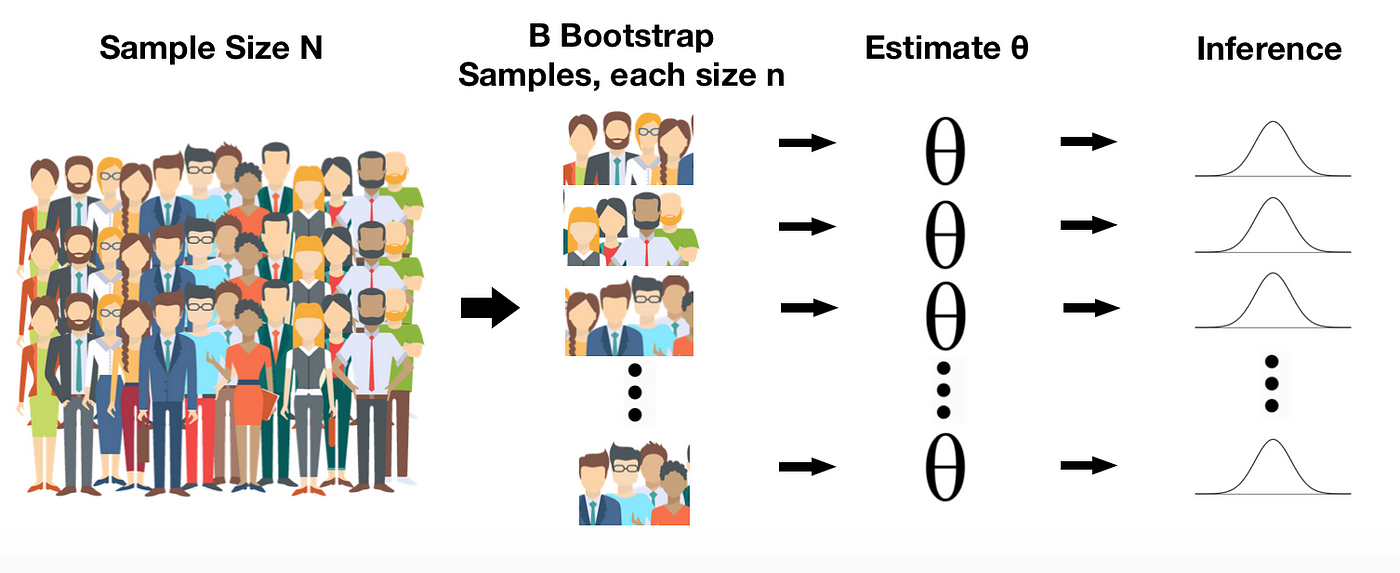
\includegraphics[width=\textwidth]{pictures/BootstrappingExample.png}
    \caption{Bootstrapping example}
    \label{fig:meinbild}
\end{figure}


Figure 2.1 provides a further illustration of the process in an abstract form. The accumulated knowledge, as illustrated in Figure 2.1, gives rise to the following process:

\begin{enumerate}
    \item \textbf{Drawing the bootstrap samples}:
    \begin{itemize}
        \item Assume we have a sample of \( n \) data points \( X = \{x_1, x_2, \ldots, x_n\} \).
        \item Draw \( B \) bootstrap samples from \( X \) with replacement. Each bootstrap sample has the same size as the original sample \( n \).
    \end{itemize}
    
    \item \textbf{Calculation of bootstraps}:
    \begin{itemize}
        \item For each of the \( B \) bootstrap samples, compute the desired statistic \( \hat{\theta}^* \) (e.g., mean, median, standard deviation).
    \end{itemize}
    
    \item \textbf{Estimation of the confidence interval}:
    \begin{itemize}
        \item Determine the \( (100 \cdot (1 - \alpha/2)) \)-th percentiles of the distribution of \( \hat{\theta}^* \) to obtain a \( (1 - \alpha) \)-confidence interval, where \( \alpha \) is the significance level.
    \end{itemize}
\end{enumerate}

\subsection{Example}
In order to provide a more illustrative example of the bootstrapping process, we will examine a fictitious case study from a practical context. 
In the field of medical research, bootstrapping represents a valuable methodology for estimating the standard error and calculating confidence intervals for a range of parameters. It is therefore appropriate to integrate this example into the medical problems sector, given that it is a topic that we always address in this course.

Let us consider a hypothetical scenario in which a research team is investigating the average efficacy of a novel pharmaceutical agent for the reduction of blood pressure in patients diagnosed with hypertension.

Steps of Bootstrapping:

\begin{enumerate}
    \item \textbf{Data collection}:
    \begin{itemize}
        \item A clinical trial was conducted by the research team, who collected a sample of 80 patients with hypertension who received the new drug.
    \end{itemize}
    
    \item \textbf{Application of the bootstrapping method}:
    \begin{itemize}
        \item \textbf{The bootstrap samples are drawn as follows:} A total of 1,000 bootstrap samples are drawn from the 80 available patient data sets.
        \item \textbf{Calculation of the bootstrap statistic:} The mean reduction in blood pressure following treatment is determined for each of the 1,000 bootstrap samples.
        \item \textbf{The estimation of the confidence interval is as follows: }The 95\% confidence interval for the mean blood pressure drop is determined by employing the 2.5\% and 97.5\% percentiles of the bootstrap mean values.
    \end{itemize}
    
    \item \textbf{Interpretation of the results}:
    \begin{itemize}
        \item The research team obtained a 95\% confidence interval for the average drop in blood pressure, for example, from 15 to 10 mmHg. This indicates that the actual mean reduction in blood pressure following treatment falls within this interval with 95\% confidence.
    \end{itemize}
\end{enumerate}

The utilisation of bootstrapping methodology allows the research team to make a well-founded assertion regarding the efficacy of the recently investigated pharmacological agent. This may subsequently result in the drug being approved or a similar outcome.
 
\section{Implementation results}
The conversion of this simple example into Python code allows the visualisation of the results. It should be noted that the values used in the code were randomly selected; this is merely an illustration of a fictitious example. 

\begin{figure}[h]
    \centering
    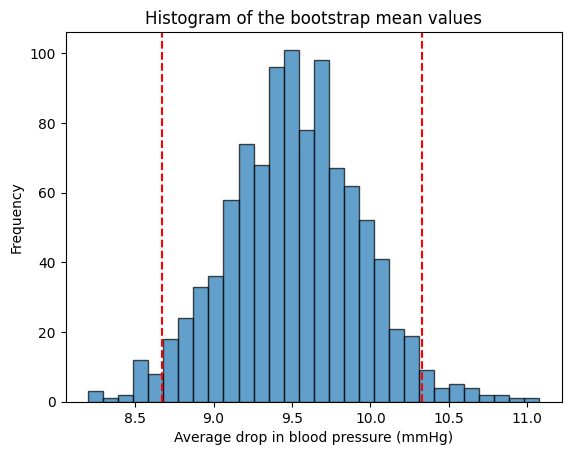
\includegraphics[width=\textwidth]{pictures/PlotBootstrappingExample.png}
    \caption{Bootstrapping example}
    \label{fig:meinbild}
\end{figure}
